% 5. Rezultati
\section{Rezultati}
\label{sec:rezultati}

Sprovedena je serija eksperimenata radi evaluacije performansi sistema EduGrader kroz više velikih jezičkih modela i konfiguracija ocenjivanja.
Tabele~\ref{tab:pra_results} i~\ref{tab:gra_results} sumiraju uporedne rezultate kroz četiri ključna pokazatelja: PCC kao meru linearne povezanosti sa ljudskim ocenama, kvadratno ponderisanu Koenovu kapu kao meru ordinalnog slaganja, odnos prosečnih ocena (prosečna ocena sistema / prosečna ocena nastavnika) kao pokazatelj sistematskog odstupanja (blagosti ili strogosti) i odnos RMSE/STDDEV kao meru relativnog odstupanja od varijabilnosti ljudskog ocenjivanja.
Tabela~\ref{tab:pra_results} prikazuje rezultate za PRA režim, dok tabela~\ref{tab:gra_results} donosi odgovarajuće rezultate za GRA režim.
Sve vrednosti su agregirani proseci izračunati nad celokupnim skupom ispitnih pitanja i instanci ocenjivanja.

\subsection{Performanse modela i analiza temperature}
\label{sec:temperatura}

\begin{table}[ht]
\centering
\caption{Metrike performansi za PRA režim kroz modele i konfiguracije strogosti.
Za modele koji podržavaju uzorkovanje evaluirane su temperature od 0{,}0 do 0{,}5; DeepSeek-Reasoner je evaluiran samo u determinističkom režimu.
Najbolji rezultati za svaku metriku i konfiguraciju strogosti označeni su podebljano.}
\label{tab:pra_results}
\resizebox{\textwidth}{!}{%
\begin{tabular}{l c ccc ccc ccc ccc}
\toprule
\textbf{Model} & \textbf{Temp} &
\multicolumn{3}{c}{\textbf{PCC}} &
\multicolumn{3}{c}{\textbf{Ponderisana kapa}} &
\multicolumn{3}{c}{\textbf{Odnos proseka}} &
\multicolumn{3}{c}{\textbf{RMSE/STDDEV}} \\
\cmidrule(lr){3-5}
\cmidrule(lr){6-8}
\cmidrule(lr){9-11}
\cmidrule(lr){12-14}
& & blag & neutr. & strog
& blag & neutr. & strog
& blag & neutr. & strog
& blag & neutr. & strog \\
\midrule

GPT-4o-mini & 0.0 & 0.76 & 0.83 & 0.77 & 0.69 & 0.82 & 0.68 & 1.22 & \textbf{1.00} & 0.75 & 0.75 & 0.55 & 0.76 \\
GPT-4o-mini & 0.1 & 0.77 & 0.84 & 0.78 & 0.72 & 0.82 & 0.68 & 1.19 & 0.99 & 0.73 & 0.71 & 0.55 & 0.76 \\
GPT-4o-mini & 0.2 & 0.79 & 0.83 & 0.77 & 0.75 & 0.81 & 0.66 & 1.16 & 0.99 & 0.72 & 0.68 & 0.55 & 0.78 \\
GPT-4o-mini & 0.3 & 0.79 & 0.83 & 0.77 & 0.74 & 0.82 & 0.67 & 1.16 & 0.98 & 0.72 & 0.67 & 0.55 & 0.78 \\
GPT-4o-mini & 0.4 & 0.78 & 0.83 & 0.78 & 0.73 & 0.82 & 0.68 & 1.19 & 0.99 & 0.73 & 0.70 & 0.55 & 0.76 \\
GPT-4o-mini & 0.5 & 0.77 & 0.84 & 0.77 & 0.70 & 0.82 & 0.68 & 1.22 & \textbf{1.00} & 0.75 & 0.74 & 0.55 & 0.75 \\

GPT-4o & 0.0 & 0.72 & 0.88 & 0.81 & 0.64 & 0.88 & 0.75 & 1.30 & 1.01 & 0.76 & 0.86 & 0.47 & 0.73 \\
GPT-4o & 0.1 & 0.73 & \textbf{0.90} & 0.84 & 0.65 & \textbf{0.90} & 0.78 & 1.30 & \textbf{1.00} & 0.78 & 0.85 & 0.45 & 0.67 \\
GPT-4o & 0.2 & 0.76 & 0.89 & 0.82 & 0.68 & 0.89 & 0.77 & 1.28 & 0.99 & 0.78 & 0.81 & 0.47 & 0.69 \\
GPT-4o & 0.3 & 0.74 & 0.89 & 0.83 & 0.67 & 0.89 & 0.78 & 1.28 & 0.99 & 0.77 & 0.83 & 0.46 & 0.68 \\
GPT-4o & 0.4 & 0.73 & 0.89 & 0.83 & 0.65 & 0.89 & 0.77 & 1.30 & \textbf{1.00} & 0.77 & 0.85 & 0.46 & 0.69 \\
GPT-4o & 0.5 & 0.71 & 0.88 & 0.82 & 0.62 & 0.88 & 0.76 & 1.31 & 1.01 & 0.77 & 0.89 & 0.48 & 0.71 \\

GPT-5.1 & 0.0 & \textbf{0.88} & \textbf{0.90} & 0.85 & \textbf{0.86} & \textbf{0.90} & 0.82 & 1.12 & 0.97 & 0.83 & \textbf{0.52} & \textbf{0.44} & 0.60 \\
GPT-5.1 & 0.1 & \textbf{0.88} & 0.89 & \textbf{0.86} & \textbf{0.86} & 0.89 & \textbf{0.83} & 1.12 & 0.96 & 0.83 & \textbf{0.52} & 0.46 & \textbf{0.59} \\
GPT-5.1 & 0.2 & \textbf{0.88} & \textbf{0.90} & 0.85 & \textbf{0.86} & 0.89 & 0.82 & \textbf{1.11} & 0.96 & 0.83 & \textbf{0.52} & 0.46 & 0.60 \\
GPT-5.1 & 0.3 & \textbf{0.88} & 0.89 & 0.85 & \textbf{0.86} & 0.89 & 0.82 & 1.12 & 0.96 & \textbf{0.84} & \textbf{0.52} & 0.46 & 0.60 \\
GPT-5.1 & 0.4 & \textbf{0.88} & 0.89 & \textbf{0.86} & \textbf{0.86} & 0.89 & \textbf{0.83} & \textbf{1.11} & 0.96 & 0.83 & \textbf{0.52} & 0.46 & \textbf{0.59} \\
GPT-5.1 & 0.5 & \textbf{0.88} & 0.89 & 0.85 & \textbf{0.86} & 0.89 & 0.82 & 1.12 & 0.97 & 0.83 & \textbf{0.52} & 0.46 & 0.60 \\

DeepSeek-Chat & 0.0 & 0.78 & 0.86 & 0.80 & 0.75 & 0.85 & 0.72 & 1.16 & 0.90 & 0.78 & 0.74 & 0.54 & 0.70 \\
DeepSeek-Chat & 0.1 & 0.78 & 0.87 & 0.80 & 0.76 & 0.85 & 0.72 & 1.16 & 0.90 & 0.78 & 0.73 & 0.53 & 0.70 \\
DeepSeek-Chat & 0.2 & 0.79 & 0.87 & 0.80 & 0.76 & 0.85 & 0.72 & 1.16 & 0.90 & 0.78 & 0.72 & 0.53 & 0.70 \\
DeepSeek-Chat & 0.3 & 0.78 & 0.86 & 0.80 & 0.76 & 0.85 & 0.72 & 1.15 & 0.90 & 0.78 & 0.73 & 0.54 & 0.70 \\
DeepSeek-Chat & 0.4 & 0.78 & 0.87 & 0.80 & 0.75 & 0.85 & 0.72 & 1.16 & 0.90 & 0.78 & 0.74 & 0.53 & 0.70 \\
DeepSeek-Chat & 0.5 & 0.78 & 0.86 & 0.80 & 0.75 & 0.85 & 0.72 & 1.16 & 0.90 & 0.77 & 0.73 & 0.53 & 0.70 \\

DeepSeek-Reasoner & 0.0 & 0.79 & 0.88 & 0.80 & 0.74 & 0.87 & 0.72 & 1.22 & 0.92 & 0.72 & 0.72 & 0.50 & 0.75 \\

\bottomrule
\end{tabular}
}
\end{table}

\begin{table}[ht]
\centering
\caption{Uticaj temperature na performanse modela GPT-5.1 u neutralnoj konfiguraciji ocenjivanja}
\label{tab:gpt51_temp}
\begin{tabular}{lccccc}
\toprule
Temperatura
& PCC
& \makecell{PCC\\p-vrednost}
& \makecell{Ponderisana\\kapa}
& \makecell{Odnos\\proseka}
& \makecell{RMSE/\\STDDEV} \\
\midrule
0.0 & \textbf{0.90} & $9.40\times10^{-247}$ & \textbf{0.90} & \textbf{0.97} & \textbf{0.44} \\
0.5 & 0.89 & $3.45\times10^{-235}$ & 0.89 & \textbf{0.97} & 0.46 \\
1.0 & 0.84 & $7.22\times10^{-168}$ & 0.84 & 0.98 & 0.55 \\
1.5 & 0.84 & $2.60\times10^{-164}$ & 0.83 & 0.98 & 0.56 \\
2.0 & 0.83 & $4.14\times10^{-160}$ & 0.83 & 0.98 & 0.57 \\
\bottomrule
\end{tabular}
\end{table}

Tabela~\ref{tab:pra_results} prikazuje rezultate evaluacije kroz različite modele i nivoe strogosti ocenjivanja (blag, neutralan i strog).
Za sve modele osim modela \emph{DeepSeek-Reasoner} eksperimenti su sprovedeni sa temperaturama od 0 do 0{,}5.
Model DeepSeek-Reasoner ne podržava uzorkovanje temperature, pa je za njega evaluirano samo determinističko zaključivanje.

U celini, GPT-5.1 pokazuje najjače ukupne performanse kroz sve evaluirane metrike.
On dosledno dostiže ili premašuje najbolje vrednosti PCC-a i ponderisane kape kroz sve konfiguracije strogosti, uz istovremeno najniže odnose RMSE/STDDEV.
Neutralna konfiguracija ocenjivanja daje najbolje rezultate kod svih modela: najviše slaganje sa ljudskim ocenjivanjem i odnose prosečnih ocena najbliže vrednosti 1{,}0.
GPT-4o ostaje konkurentan, naročito u neutralnoj konfiguraciji, dok GPT-4o-mini i DeepSeek-Chat pokazuju nešto niže slaganje i veću varijabilnost izvan neutralne konfiguracije.

Na osnovu rezultata iz tabele~\ref{tab:pra_results}, za dalju analizu temperature izabrani su GPT-5.1 i neutralna konfiguracija ocenjivanja.
Tabela~\ref{tab:gpt51_temp} stoga prikazuje širi opseg temperatura i dodatno navodi odgovarajuće p-vrednosti PCC-a.
Sve prikazane p-vrednosti su izuzetno male ($p \ll 0{,}001$), što ukazuje da su korelacije između ocena modela i ljudskih ocena visoko statistički značajne.
Dodatna analiza temperature za GPT-5.1 u neutralnoj konfiguraciji pokazuje da performanse ostaju veoma stabilne do temperature 0{,}5: PCC opada tek neznatno, sa 0{,}90 na 0{,}89, odnos prosečnih ocena ostaje blizu 1{,}0, a RMSE/STDDEV raste samo marginalno.
Na višim temperaturama (1{,}0--2{,}0) slaganje sa ljudskim ocenjivanjem postepeno opada, što ukazuje da su niže temperature pogodnije za dosledno automatsko ocenjivanje.

Tabela~\ref{tab:gra_results} prikazuje rezultate za \textbf{GRA} režim, u kome referentne odgovore automatski generiše jezički model umesto nastavnika.
Za GRA eksperiment korišćena je fiksna temperatura 0{,}2 za sve modele (osim modela DeepSeek-Reasoner, koji koristi determinističko zaključivanje).
Očekivano, rezultati u GRA režimu su generalno niži od onih dobijenih sa referentnim odgovorima nastavnika.
Ovaj pad performansi odražava dodatnu neizvesnost koju unose automatski generisani referentni odgovori, koji se mogu razlikovati po strukturi, formulaciji ili nivou detalja od rešenja koje je nastavnik imao na umu.
Uprkos tome, modeli i dalje postižu umereno do snažno slaganje sa ljudskim ocenjivanjem, što pokazuje da sistem ostaje efikasan i kada se referentni odgovori generišu automatski.
Među evaluiranim modelima, GPT-5.1 ponovo postiže najjače ukupne performanse, dostižući ili premašujući najbolje vrednosti PCC-a i kape kroz konfiguracije i dajući najniže odnose RMSE/STDDEV.
Ovo sugeriše da su jači modeli za rezonovanje sposobniji i da generišu prikladne referentne odgovore i da studentske odgovore ocene u odnosu na njih.
Iako je slaganje sa ljudskim ocenjivanjem nešto niže nego u PRA režimu, rezultati pokazuju da EduGrader ostaje robustan i praktično upotrebljiv čak i u potpuno automatizovanom toku sa generisanjem referentnih odgovora.

\begin{table}[ht]
\centering
\caption{Metrike performansi za GRA režim}
\label{tab:gra_results}
\resizebox{\textwidth}{!}{
\begin{tabular}{l ccc ccc ccc ccc}
\toprule
\textbf{Model} &
\multicolumn{3}{c}{\textbf{PCC}} &
\multicolumn{3}{c}{\textbf{Ponderisana kapa}} &
\multicolumn{3}{c}{\textbf{Odnos proseka}} &
\multicolumn{3}{c}{\textbf{RMSE/STDDEV}} \\
\cmidrule(lr){2-4}
\cmidrule(lr){5-7}
\cmidrule(lr){8-10}
\cmidrule(lr){11-13}
& blag & neutr. & strog
& blag & neutr. & strog
& blag & neutr. & strog
& blag & neutr. & strog \\
\midrule
GPT-4o-mini       & 0.71 & 0.70 & 0.67 & 0.67 & 0.64 & 0.41 & 1.18 & 0.84 & 0.56 & 0.76 & 0.76 & 1.03 \\
GPT-4o            & 0.71 & 0.80 & 0.71 & 0.64 & 0.79 & 0.54 & 1.26 & 0.94 & 0.59 & 0.84 & 0.62 & 0.97 \\
GPT-5.1           & \textbf{0.82} & \textbf{0.80} & \textbf{0.73} & \textbf{0.81} & \textbf{0.78} & \textbf{0.63} & 1.08 & 0.87 & \textbf{0.69} & \textbf{0.59} & \textbf{0.65} & \textbf{0.87} \\
DeepSeek-Chat     & 0.71 & 0.76 & 0.69 & 0.68 & 0.71 & 0.51 & 1.16 & 0.79 & 0.63 & 0.84 & 0.75 & 0.94 \\
DeepSeek-Reasoner & 0.77 & 0.79 & 0.64 & 0.73 & 0.76 & 0.47 & 1.19 & 0.81 & 0.55 & 0.72 & 0.68 & 1.08 \\
\bottomrule
\end{tabular}
}
\end{table}

\subsection{Poređenje PRA i GRA režima kroz modele i nivoe strogosti}
\label{sec:pra-vs-gra}

Kroz sve evaluirane modele i konfiguracije strogosti, PRA režim dosledno nadmašuje GRA režim.
PRA postavka postiže više korelacije sa ljudskim ocenama, jače ordinalno slaganje (više vrednosti kape) i niže normalizovane odnose greške.
Ovi rezultati potvrđuju da obezbeđivanje referentnih odgovora od strane nastavnika suštinski poboljšava stabilnost ocenjivanja i usklađenost sa ljudskim ocenjivačima.

\subsubsection{Korelacija sa ljudskim ocenjivanjem}

U PRA režimu, GPT-5.1 postiže najvišu korelaciju sa ljudskim ocenjivanjem kroz sve konfiguracije, dostižući vrednosti PCC-a od približno 0{,}88--0{,}90.
GPT-4o ga prati u stopu, naročito u neutralnoj konfiguraciji (PCC $= 0{,}90$).
DeepSeek-Chat i GPT-4o-mini postižu umereno visoke korelacije, sa najjačim vrednostima u neutralnoj konfiguraciji (do 0{,}87 odnosno 0{,}84), ali primetno nižim korelacijama u blagoj i strogoj konfiguraciji.

Prelaskom na GRA režim korelacije opadaju kod svih modela.
GPT-5.1 ostaje najjači model (PCC do 0{,}82), a slede DeepSeek-Reasoner i GPT-4o, dok GPT-4o-mini i DeepSeek-Chat pokazuju nešto niže vrednosti korelacije.

\subsubsection{Slaganje sa ljudskim ocenjivanjem}

Kvadratno ponderisana kapa pruža perspektivu orijentisanu na slaganje, komplementarnu PCC-u.
U PRA režimu, GPT-5.1 postiže najviše slaganje sa ljudskim ocenjivanjem (kapa do 0{,}90), a slede ga GPT-4o i DeepSeek-Chat.
Slaganje opada u GRA režimu kod svih modela, što potvrđuje da automatski generisani referentni odgovori unose dodatnu varijabilnost u ocenjivanje.

\subsubsection{Odnos prosečnih ocena i sistematsko odstupanje}

Vrednosti odnosa prosečnih ocena ukazuju na umereno sistematsko odstupanje kroz modele.
GPT-5.1 ostaje najbliži prosecima ljudskog ocenjivanja, sa odnosima blizu 1{,}0 u neutralnoj konfiguraciji (0{,}96--0{,}97).
GPT-4o i GPT-4o-mini pokazuju nešto blaže ocenjivanje u pojedinim konfiguracijama (odnosi iznad 1{,}2 u blagoj konfiguraciji).
DeepSeek-Chat i DeepSeek-Reasoner generalno daju nešto niže odnose u neutralnoj i strogoj konfiguraciji, što ukazuje na konzervativniju tendenciju ocenjivanja u odnosu na ljudske ocenjivače.

\subsubsection{Odnosi greške i stabilnost}

Rezultati RMSE/STDDEV dodatno ističu razlike u stabilnosti ocenjivanja.
GPT-5.1 postiže najniže normalizovane odnose greške u većini konfiguracija (do 0{,}44), što ukazuje na najbliže poklapanje sa prirodnom varijabilnošću ljudskog ocenjivanja.
GPT-4o takođe postiže dobre rezultate, naročito u neutralnoj i strogoj konfiguraciji, gde RMSE/STDDEV ostaje relativno nizak; blaga konfiguracija, međutim, pokazuje primetno više odnose greške.
GPT-4o-mini i DeepSeek-Chat pokazuju veću varijabilnost, naročito u strožim konfiguracijama, gde se RMSE/STDDEV približava vrednosti 0{,}75 ili je premašuje.
DeepSeek-Reasoner ostaje konkurentan, ali nešto manje stabilan od modela GPT-5.1.

\subsubsection{Uporedni pregled performansi}

Kroz metrike korelacije, slaganja, sistematskog odstupanja i greške izdvaja se nekoliko zaključaka:

\begin{itemize}
    \item GPT-5.1 je ukupno najjači model: postiže najvišu korelaciju i slaganje sa ljudskim ocenjivačima, uz najniže odnose greške.
    \item GPT-4o nudi konkurentne performanse i stabilno ponašanje kroz različite temperature.
    \item GPT-4o-mini pruža povoljan odnos cene i performansi, postižući razumnu korelaciju uz umerene nivoe greške.
    \item DeepSeek-Chat i DeepSeek-Reasoner ostaju upotrebljive alternative, ali pokazuju nešto slabiju usklađenost sa ljudskim ocenjivanjem u poređenju sa GPT-5.1.
\end{itemize}

U celini, rezultati potvrđuju tri ključna nalaza:
\begin{itemize}
    \item obezbeđivanje referentnih odgovora nastavnika (PRA) značajno poboljšava pouzdanost ocenjivanja;
    \item sposobniji modeli za rezonovanje postižu jače slaganje sa ljudskim ocenjivačima;
    \item zaključivanje na niskim temperaturama daje najstabilnije ponašanje automatskog ocenjivanja.
\end{itemize}

\subsection{Bland--Altmanova analiza slaganja}
\label{sec:bland-altman}

Pored metrika zasnovanih na korelaciji, slaganje između ocena jezičkih modela i ljudskih ocena dodatno je ispitano Bland--Altmanovom analizom~\cite{mansournia2021bland}.
Ova perspektiva je posebno relevantna u svetlu novijih studija koje porede ocenjivanje generativnom veštačkom inteligencijom sa ljudskom evaluacijom eseja i odgovora otvorenog tipa~\cite{olivos2025assessing,wetzler2025grading}.
Za svaki ocenjeni studentski odgovor, dijagram prikazuje prosek dve ocene na x-osi i njihovu razliku (LLM $-$ nastavnik) na y-osi.
Horizontalna puna linija označava prosečnu razliku (sistematsko odstupanje), dok isprekidane linije predstavljaju 95\% granice slaganja (prosek $\pm$ 1{,}96 SD).

Slika~\ref{fig:ba_pra} prikazuje Bland--Altmanove dijagrame za sve evaluirane modele u PRA režimu ocenjivanja.
U neutralnoj konfiguraciji, GPT-5.1 pokazuje najmanje prosečno odstupanje (blizu nule) i najuže granice slaganja, što potvrđuje najjaču usklađenost sa ljudskim ocenjivanjem.
Blaga konfiguracija generalno pomera prosečnu razliku naviše (pozitivno odstupanje --- model ocenjuje više od nastavnika), dok je stroga konfiguracija pomera naniže.
Ovi obrasci su u skladu sa rezultatima odnosa prosečnih ocena iz tabele~\ref{tab:pra_results}.

Slika~\ref{fig:ba_gra} prikazuje odgovarajuće Bland--Altmanove dijagrame za GRA režim.
U poređenju sa PRA režimom, granice slaganja su šire kod svih modela, što odražava dodatnu varijabilnost koju unose automatski generisani referentni odgovori.
Uprkos tome, GPT-5.1 ponovo postiže najkompaktnije granice slaganja.

\begin{figure}[ht!]
\centering
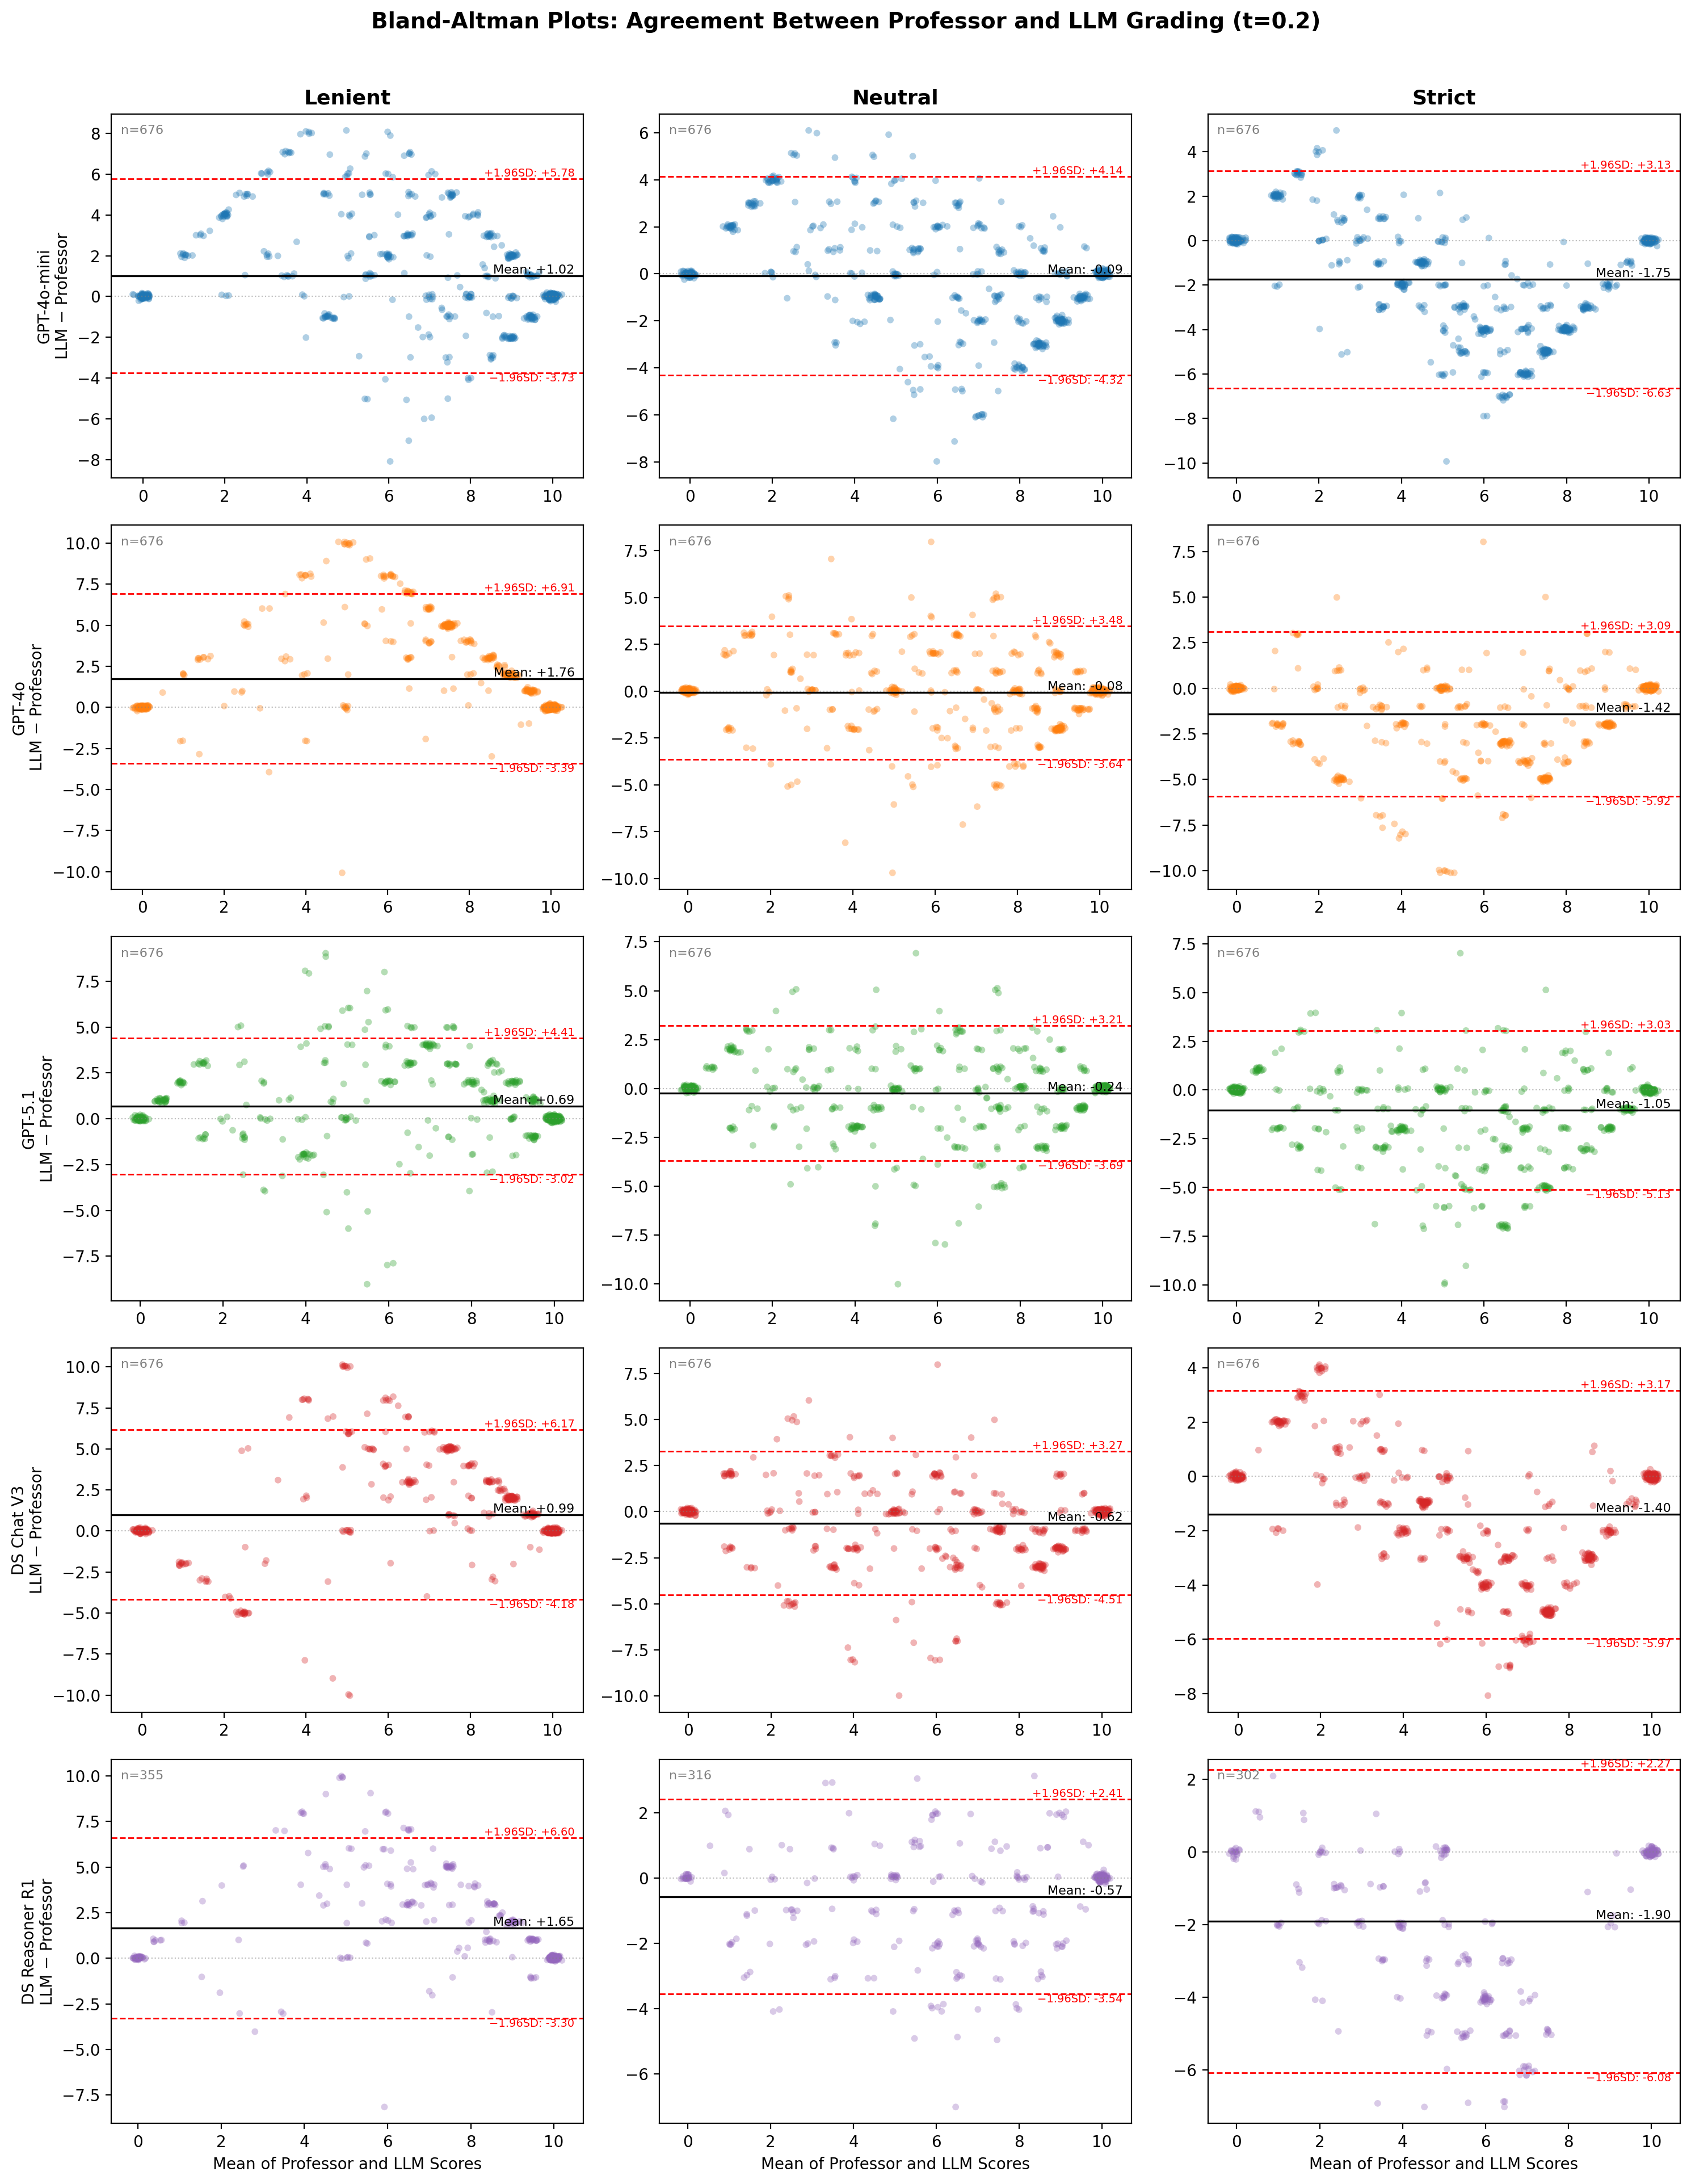
\includegraphics[width=\textwidth]{figures/bland_altman_pra.png}
\caption{Bland--Altmanovi dijagrami za PRA režim kroz sve modele i konfiguracije strogosti ($t=0{,}2$).
Svaka tačka predstavlja jedan ocenjeni studentski odgovor.}
\label{fig:ba_pra}
\end{figure}

\begin{figure}[ht!]
\centering
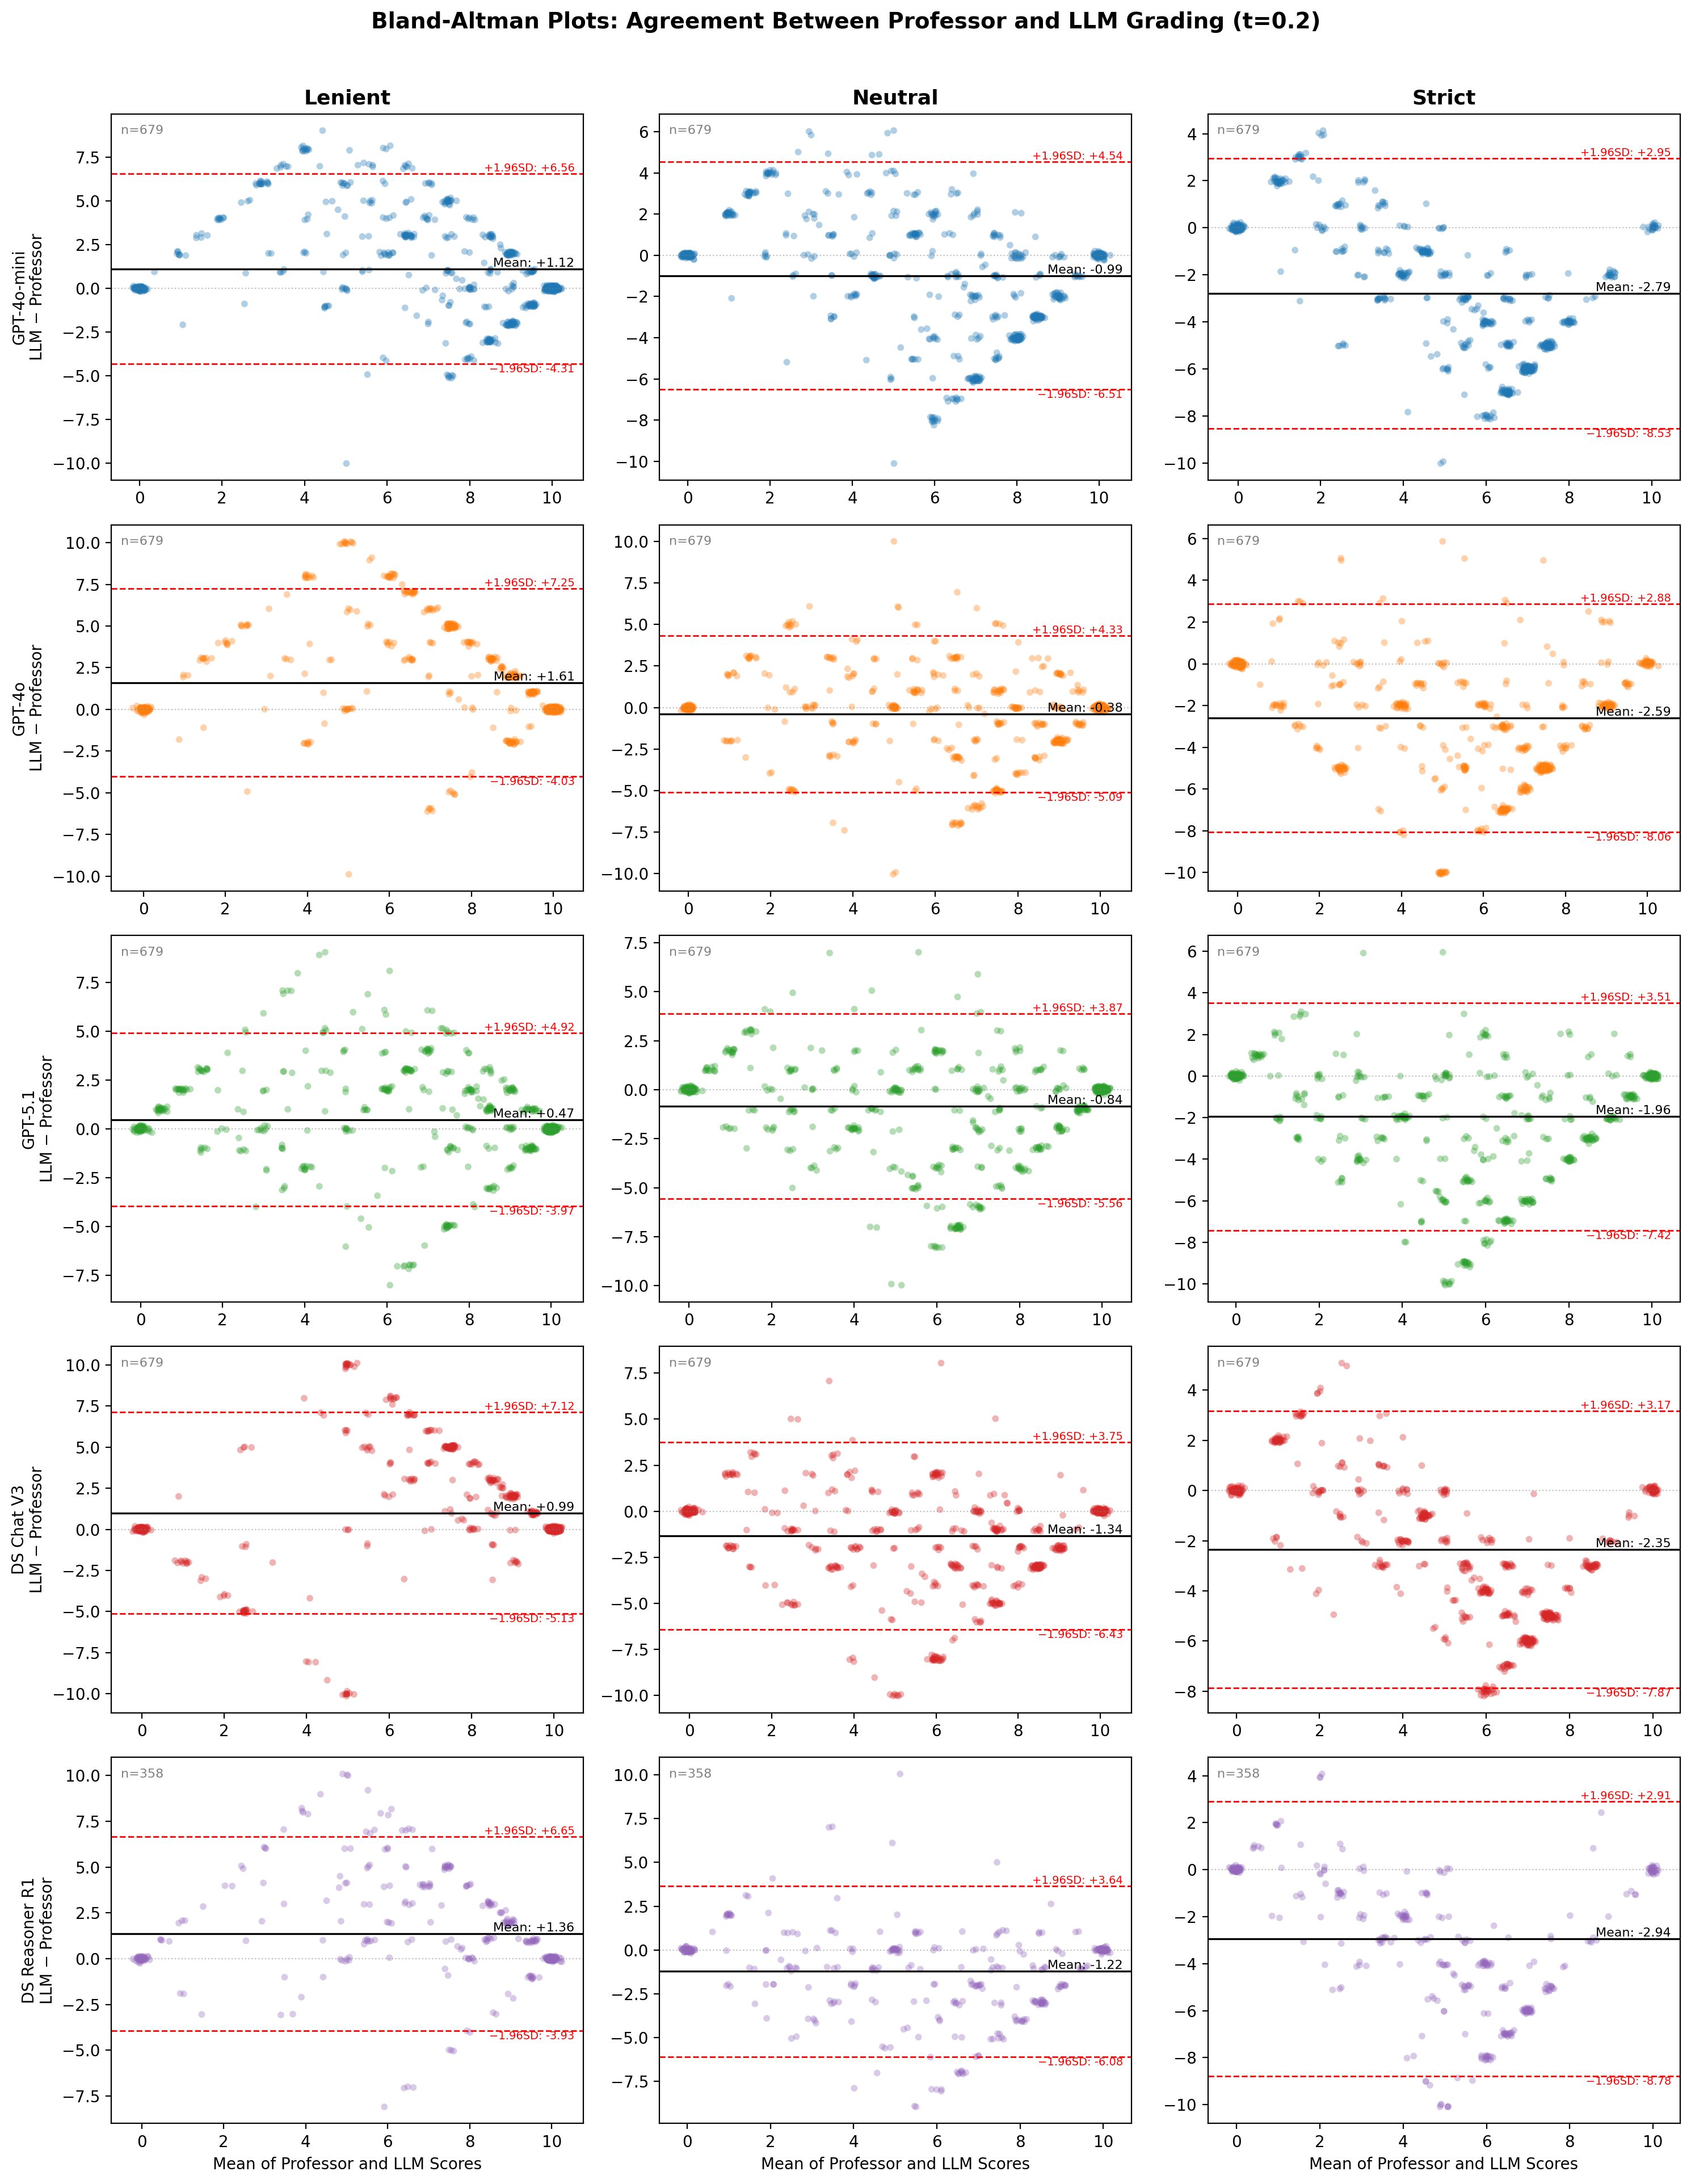
\includegraphics[width=\textwidth]{figures/bland_altman_gra.png}
\caption{Bland--Altmanovi dijagrami za GRA režim kroz sve modele i konfiguracije strogosti ($t=0{,}2$).}
\label{fig:ba_gra}
\end{figure}

\subsection{Analiza PCC-a po skupovima podataka}
\label{sec:cross-dataset}

Tabele~\ref{tab:pcc-reference-best} i~\ref{tab:pcc-generated-best} prikazuju vrednosti PCC-a kroz sve skupove podataka za PRA odnosno GRA ocenjivanje, koristeći neutralnu konfiguraciju za svaki model.
To omogućava poređenje modela u njihovim optimalnim konfiguracijama, umesto u jednoj fiksnoj globalnoj postavci.

Primetna razlika između PRA i GRA rezultata javlja se na kursevima gde se očekuje veoma kratak i precizan studentski odgovor, kao što su WP i TSW.
Na ovim skupovima podataka vrednosti PCC-a za GRA znatno opadaju u odnosu na PRA (tabela~\ref{tab:pcc-reference-best} naspram tabele~\ref{tab:pcc-generated-best}).
Jedan od razloga je taj što automatski generisani referentni odgovori teže da budu znatno duži i opisniji od sažetih rešenja koja daje nastavnik.
Kao posledica, model često dodeljuje visoke ocene odgovorima koji ispravno opisuju traženi postupak, ali ga zapravo ne izvršavaju.
Nasuprot tome, nastavnik je takve odgovore ocenjivao strogo i po pravilu dodeljivao nula poena kada tražena radnja nije sprovedena.
Ovaj raskorak između opisne i proceduralne tačnosti smanjuje slaganje sa ljudskim ocenjivanjem.

Ovakvo ponašanje može se ublažiti uključivanjem kratke napomene nastavnika koja eksplicitno naglašava da li je tačno objašnjenje samo po sebi dovoljno ili student mora u potpunosti da izvrši traženi zadatak.
Takvo usmerenje pomaže modelu da kriterijume ocenjivanja bolje uskladi sa očekivanjima nastavnika.

Kod skupova podataka gde se očekuju duži, opisniji odgovori (npr.\ DDS, DM i HTML5), razlike između PRA i GRA su znatno manje.
U tim slučajevima generisani referentni odgovori po strukturi i nivou detalja liče na odgovore nastavnika, što vodi sličnom ponašanju pri ocenjivanju i uporedivim vrednostima PCC-a u oba režima.

\begin{table}[ht]
\centering
\caption{PCC kroz sve skupove podataka za PRA režim (neutralna konfiguracija, temperatura 0{,}2; DeepSeek-Reasoner ne podržava podešavanje temperature)}
\label{tab:pcc-reference-best}
\resizebox{\columnwidth}{!}{%
\begin{tabular}{lccccc}
\toprule
\textbf{Skup podataka} & \textbf{DeepSeek-Chat} & \textbf{DeepSeek-Reasoner} & \textbf{GPT-4o} & \textbf{GPT-4o-mini} & \textbf{GPT-5.1} \\
\midrule
Prog 2 & 0.86 & 0.88 & \textbf{0.89} & 0.84 & \textbf{0.89} \\
TSW    & \textbf{0.94} & 0.88 & 0.92 & 0.91 & \textbf{0.94} \\
WP     & 0.78 & 0.67 & 0.78 & 0.77 & \textbf{0.87} \\
DDS    & 0.91 & 0.88 & 0.77 & \textbf{0.95} & 0.92 \\
HTML5  & 0.96 & 0.93 & \textbf{0.97} & 0.96 & \textbf{0.97} \\
DM     & 0.82 & 0.84 & 0.87 & 0.75 & \textbf{0.91} \\
\bottomrule
\end{tabular}
}
\end{table}

\begin{table}[ht]
\centering
\caption{Najbolji PCC kroz sve skupove podataka za GRA režim (temperatura 0{,}2; DeepSeek-Reasoner koristi temperaturu 0 jer ne podržava podešavanje temperature)}
\label{tab:pcc-generated-best}
\resizebox{\columnwidth}{!}{%
\begin{tabular}{lccccc}
\toprule
\textbf{Skup podataka} & \textbf{DeepSeek-Chat} & \textbf{DeepSeek-Reasoner} & \textbf{GPT-4o} & \textbf{GPT-4o-mini} & \textbf{GPT-5.1} \\
\midrule
Prog 2 & 0.78 & 0.81 & 0.80 & 0.76 & \textbf{0.84} \\
TSW    & 0.51 & 0.78 & \textbf{0.84} & 0.64 & 0.57 \\
WP     & 0.62 & 0.66 & \textbf{0.82} & 0.80 & 0.76 \\
DDS    & 0.81 & 0.66 & \textbf{0.89} & 0.87 & \textbf{0.89} \\
HTML5  & 0.95 & 0.92 & 0.98 & 0.97 & \textbf{0.99} \\
DM     & 0.82 & 0.83 & 0.85 & 0.75 & \textbf{0.92} \\
\bottomrule
\end{tabular}
}
\end{table}

\subsection{Stabilnost ocenjivanja kroz višestruka pokretanja}
\label{sec:stabilnost}

Budući da su izlazi velikih jezičkih modela inherentno stohastički, stabilnost ocenjivanja dodatno je procenjena ponavljanjem istog zadatka ocenjivanja tri nezavisna puta, koristeći GPT-5.1 sa temperaturom 0{,}2 i podrazumevanim (neutralnim) promptom strogosti.
Tabela~\ref{tab:variability} sumira rezultate.

Nad svih 686 pitanja, agregirane metrike pokazale su zanemarljivu varijaciju između pokretanja: PCC $= 0{,}899 \pm 0{,}002$, ponderisana kapa $= 0{,}896 \pm 0{,}002$, odnos prosečnih ocena $= 0{,}962 \pm 0{,}002$ i RMSE/STDDEV $= 0{,}448 \pm 0{,}003$.
Na nivou pojedinačnih pitanja, 82\% ocena bilo je identično u sva tri pokretanja, a 97\% se razlikovalo za najviše 1 poen na skali 0--10, uz prosečnu maksimalnu razliku od 0{,}21 poena.

Na nivou skupova podataka, varijabilnost je ostala niska u svim slučajevima, sa najmanjim standardnim devijacijama kod najstabilnijih podskupova i nešto višom varijabilnošću kod manjih skupova podataka.

\begin{table}[ht]
\centering
\caption{Analiza varijabilnosti ocenjivanja modela GPT-5.1 za PRA režim kroz tri nezavisna pokretanja ($t=0{,}2$, podrazumevana strogost).
Svako polje prikazuje prosek $\pm$ standardnu devijaciju nad 3 pokretanja.}
\label{tab:variability}
\resizebox{\columnwidth}{!}{%
\begin{tabular}{lcccc}
\toprule
\textbf{Skup podataka} & \textbf{PCC} & \textbf{Ponderisana kapa} & \textbf{Odnos proseka} & \textbf{RMSE/STDDEV} \\
\midrule
Prog 2 & 0.892 $\pm$ 0.002 & 0.888 $\pm$ 0.002 & 0.941 $\pm$ 0.002 & 0.464 $\pm$ 0.004 \\
TSW    & 0.953 $\pm$ 0.006 & 0.886 $\pm$ 0.013 & 0.979 $\pm$ 0.002 & 0.328 $\pm$ 0.026 \\
WP     & 0.855 $\pm$ 0.006 & 0.747 $\pm$ 0.011 & 0.930 $\pm$ 0.002 & 0.694 $\pm$ 0.030 \\
DDS    & 0.882 $\pm$ 0.016 & 0.823 $\pm$ 0.034 & 0.869 $\pm$ 0.010 & 0.622 $\pm$ 0.026 \\
HTML5  & 0.969 $\pm$ 0.004 & 0.959 $\pm$ 0.006 & 0.898 $\pm$ 0.008 & 0.311 $\pm$ 0.019 \\
DM     & 0.915 $\pm$ 0.005 & 0.894 $\pm$ 0.005 & 1.109 $\pm$ 0.003 & 0.466 $\pm$ 0.012 \\
\midrule
SVI    & 0.899 $\pm$ 0.002 & 0.896 $\pm$ 0.002 & 0.962 $\pm$ 0.002 & 0.448 $\pm$ 0.003 \\
\bottomrule
\end{tabular}
}
\end{table}
